\section{Combining Control and Sensory Feedback}
After the subject was trained in understanding one of the feedback schemes, the sensory feedback was combined with prosthetic control. Similar to the control block of the study, see \subref{sec:meth:contraintest}, the subject would go through a familiarization phase before undergoing evaluation tests.  These stages will be explained in the following sections. An illustration of the full experiment setup used in this trial can be seen in \figref{fig:meth:setup}.

\subsection{Familiarization}
This stage was similar to the second stage control training, see \secref{sec:meth:contrain}, with the addition of receiving sensory feedback. The subject was instructed in getting reacquainted with the prosthetic control, while adapting further to the feedback related to the various prosthesis states as well the transitions felt when changing prosthesis state. These focus point were assessed most beneficial to train in order to perform well in the final evaluation test. The duration of the familiarization phase was three minutes.

\subsection{Final Evaluation Test}
This evaluation test was similar to the evaluation test from the control step, see \secref{sec:meth:contest}, with the addition of receiving sensory feedback. In this test, the prosthesis state would, however, not be visualized. Thus, the subject had to use the sensory feedback to determine the prosthesis state and reach the highlighted targets. The target reaching test was performed two times consecutively. Again the completion rate, time to reach a target and length travelled to reach a target were extracted for performance evaluation.

\begin{figure}[H]                 
	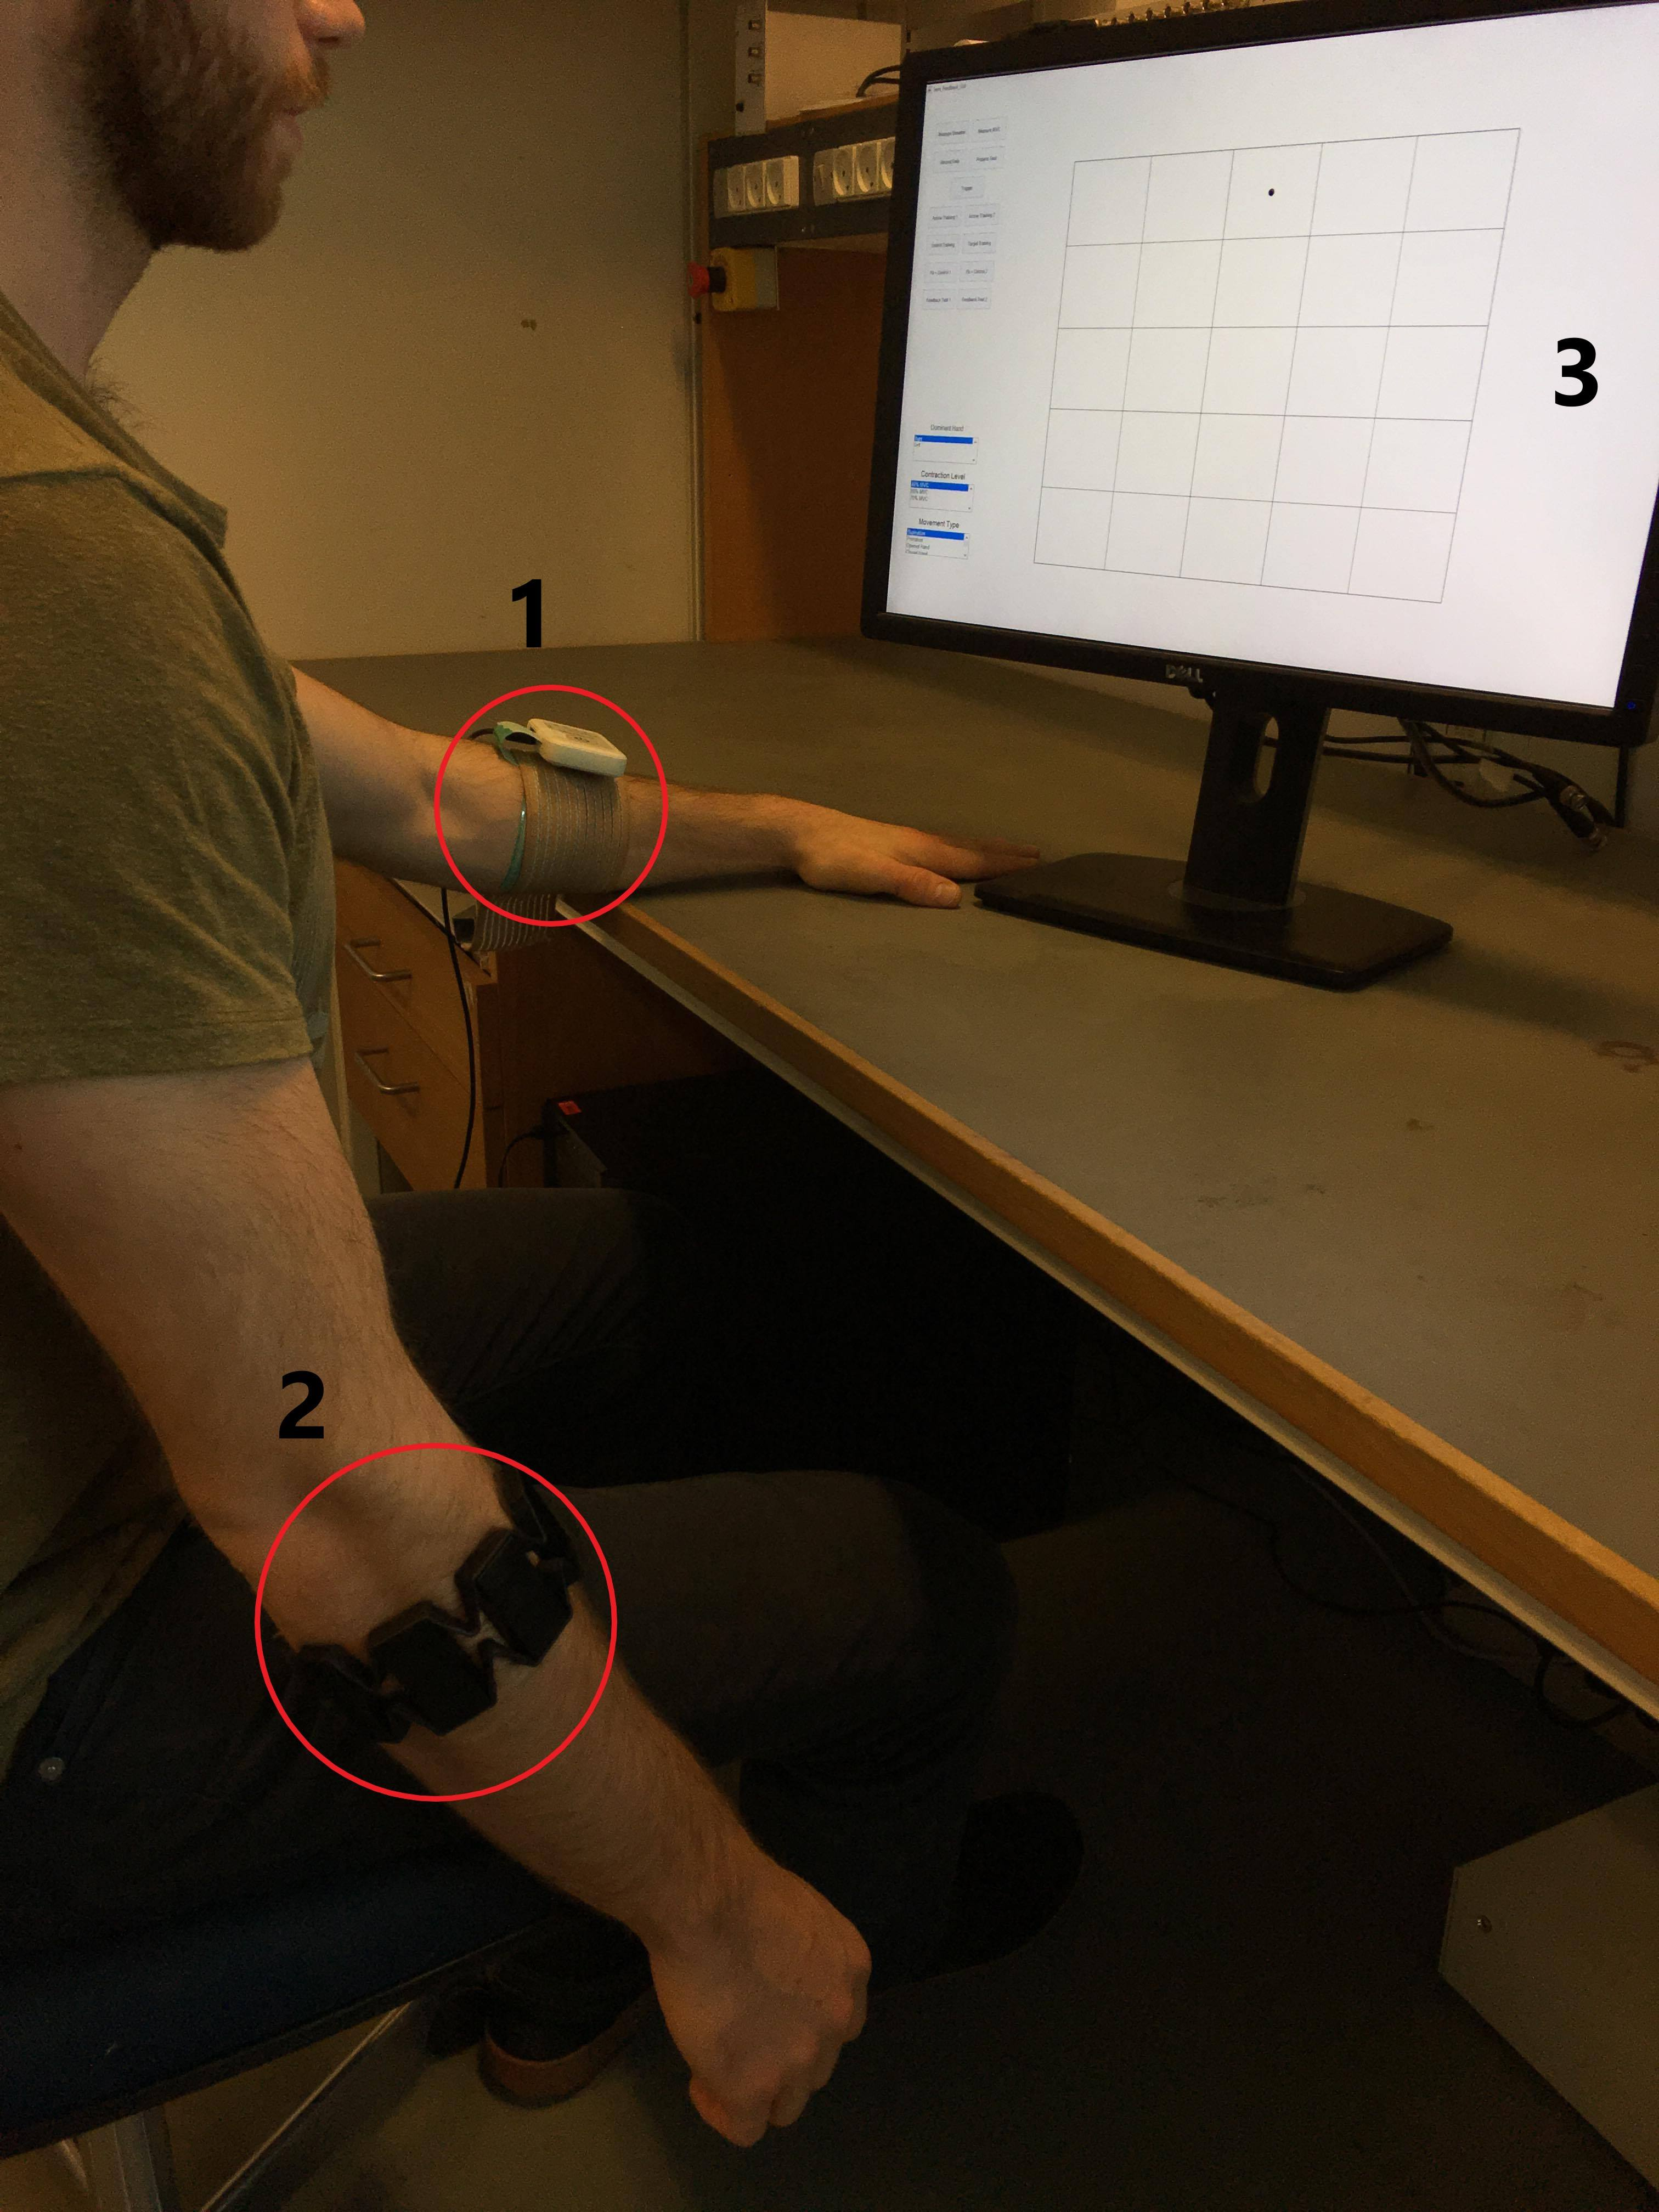
\includegraphics[width=0.8\textwidth]{figures/setupimg}  
	\caption{Image of the experimental setup. 1) is the stimulation device with the stimulation electrode placed under the brown armband, 2) is the electrode armband used to record EMG signals and 3) is the computer screen used to guide the subject and display tasks.} 
	\label{fig:meth:setup} 
\end{figure}